\section{Constrained Stochastic Sampling with Semantic Gravity}
\label{sec:constrained-sampling}

This section establishes the theoretical foundations for constrained stochastic sampling within semantic coordinate spaces, implementing controlled random walks subject to semantic gravity constraints. The methodology constitutes the Moon Landing Algorithm's second processing layer, enabling systematic exploration of compressed coordinate manifolds through physically-motivated sampling dynamics.

\subsection{Semantic Gravity Field Formulation}

\begin{definition}[Semantic Gravity Field]
Let $\mathcal{U}$ represent a semantic coordinate space equipped with potential energy function $U_s: \mathcal{U} \to \mathbb{R}$. The semantic gravity field $\mathbf{g}_s: \mathcal{U} \to \mathbb{R}^d$ is defined as:
\begin{equation}
\mathbf{g}_s(\mathbf{r}) = -\nabla U_s(\mathbf{r})
\label{eq:semantic-gravity}
\end{equation}
where $\mathbf{r} \in \mathcal{U}$ denotes position coordinates and $\nabla$ represents the gradient operator.
\end{definition}

The potential energy function incorporates multiple semantic zones $\{\mathcal{Z}_j\}_{j=1}^M$:

\begin{equation}
U_s(\mathbf{r}) = \sum_{j=1}^M U_j(\mathbf{r}) = \sum_{j=1}^M \frac{\epsilon_j}{\|\mathbf{r} - \mathbf{c}_j\| + \delta}
\label{eq:semantic-potential}
\end{equation}

where $\mathbf{c}_j \in \mathcal{U}$ represents the center of semantic zone $j$, $\epsilon_j \in \mathbb{R}$ denotes zone strength (positive for attractive, negative for repulsive), and $\delta > 0$ prevents singularities.

The resulting gravity force field exhibits the form:

\begin{equation}
\mathbf{g}_s(\mathbf{r}) = \sum_{j=1}^M \frac{\epsilon_j}{(\|\mathbf{r} - \mathbf{c}_j\| + \delta)^2} \frac{\mathbf{r} - \mathbf{c}_j}{\|\mathbf{r} - \mathbf{c}_j\|}
\label{eq:gravity-force}
\end{equation}

\subsection{Fuzzy Window Aperture Functions}

\begin{definition}[Multidimensional Fuzzy Window]
The fuzzy window aperture function $\psi: \mathcal{U} \to [0,1]$ implements smooth spatial filtering through Gaussian-weighted apertures:
\begin{equation}
\psi(\mathbf{r}) = \prod_{k=1}^d \psi_k(r_k) = \prod_{k=1}^d \exp\left(-\frac{(r_k - c_k)^2}{2\sigma_k^2}\right)
\label{eq:fuzzy-window}
\end{equation}
where $c_k$ and $\sigma_k$ represent the center and width parameters for dimension $k$.
\end{definition}

The composite sample weighting function combines multiple fuzzy windows:

\begin{equation}
w(\mathbf{r}) = \prod_{j=1}^J \psi_j(\mathbf{r}) = \prod_{j=1}^J \prod_{k=1}^d \exp\left(-\frac{(r_k - c_{j,k})^2}{2\sigma_{j,k}^2}\right)
\label{eq:composite-weight}
\end{equation}

\subsection{Constrained Step Size Dynamics}

The fundamental constraint governing stochastic motion establishes maximum step size as inversely proportional to local gravity magnitude:

\begin{equation}
\Delta r_{\max}(\mathbf{r}) = \frac{v_0}{\|\mathbf{g}_s(\mathbf{r})\| + \epsilon_g}
\label{eq:step-constraint}
\end{equation}

where $v_0 > 0$ represents the processing velocity parameter and $\epsilon_g > 0$ prevents division by zero in regions of negligible gravity.

\begin{definition}[Constrained Stochastic Process]
The constrained random walk evolves according to the discrete-time stochastic process:
\begin{align}
\mathbf{r}_{t+1} &= \mathbf{r}_t + \boldsymbol{\xi}_t \label{eq:stochastic-evolution}\\
\boldsymbol{\xi}_t &\sim \mathcal{N}_{\text{trunc}}\left(\mathbf{0}, \sigma_t^2 \mathbf{I}_d, \mathcal{B}_t\right) \label{eq:truncated-normal}
\end{align}
where $\mathcal{N}_{\text{trunc}}$ denotes the truncated multivariate normal distribution, $\sigma_t = \Delta r_{\max}(\mathbf{r}_t)/3$, and $\mathcal{B}_t = \{\boldsymbol{\xi}: \|\boldsymbol{\xi}\| \leq \Delta r_{\max}(\mathbf{r}_t)\}$ represents the constraint set.
\end{definition}

\subsection{Sampling Algorithm and Convergence Properties}

The constrained stochastic sampling algorithm proceeds through iterative "pogo stick jumps":

\begin{algorithm}[H]
\caption{Constrained Stochastic Sampling}
\begin{algorithmic}[1]
\STATE Initialize $\mathbf{r}_0 \in \mathcal{U}$, set $t = 0$
\WHILE{$t < T_{\max}$}
    \STATE Compute $\|\mathbf{g}_s(\mathbf{r}_t)\|$
    \STATE Calculate $\Delta r_{\max}(\mathbf{r}_t)$ via Equation~\eqref{eq:step-constraint}
    \STATE Sample $\boldsymbol{\xi}_t \sim \mathcal{N}_{\text{trunc}}(\mathbf{0}, (\Delta r_{\max}/3)^2 \mathbf{I}_d, \mathcal{B}_t)$
    \STATE Update $\mathbf{r}_{t+1} = \mathbf{r}_t + \boldsymbol{\xi}_t$
    \STATE Calculate $w(\mathbf{r}_{t+1})$ via Equation~\eqref{eq:composite-weight}
    \STATE Store sample $(\mathbf{r}_{t+1}, w(\mathbf{r}_{t+1}))$
    \STATE $t \leftarrow t + 1$
\ENDWHILE
\end{algorithmic}
\end{algorithm}

\subsection{Effective Sample Size and Sampling Efficiency}

The effective sample size accounts for weighted sampling:

\begin{equation}
N_{\text{eff}} = \frac{\left(\sum_{i=1}^N w_i\right)^2}{\sum_{i=1}^N w_i^2}
\label{eq:effective-sample-size-constrained}
\end{equation}

\begin{definition}[Sampling Efficiency]
The sampling efficiency $\eta$ quantifies the ratio of effective to total samples:
\begin{equation}
\eta = \frac{N_{\text{eff}}}{N} = \frac{\left(\sum_{i=1}^N w_i\right)^2}{N \sum_{i=1}^N w_i^2}
\label{eq:sampling-efficiency}
\end{equation}
\end{definition}

\subsection{Theoretical Convergence Analysis}

\begin{theorem}[Ergodicity of Constrained Process]
Under conditions of bounded gravity field $\|\mathbf{g}_s(\mathbf{r})\| < G_{\max} < \infty$ and connected domain $\mathcal{U}$, the constrained stochastic process \eqref{eq:stochastic-evolution} is ergodic with stationary distribution $\pi(\mathbf{r}) \propto w(\mathbf{r}) \exp(-\beta U_s(\mathbf{r}))$ where $\beta^{-1}$ represents the effective temperature.
\end{theorem}

\begin{proof}[Sketch]
The proof follows from establishing irreducibility through positive probability transitions between any two states within finite time, and aperiodicity through the continuous nature of the truncated normal perturbations. The bounded step sizes ensure finite expected return times to compact sets.
\end{proof}

\subsection{Computational Complexity and Scalability}

The computational complexity per sampling step scales as $\mathcal{O}(M \cdot d + J \cdot d)$ where $M$ represents the number of semantic gravity zones and $J$ the number of fuzzy windows. The truncated normal sampling requires $\mathcal{O}(d^2)$ operations for covariance matrix operations, yielding total complexity $\mathcal{O}(d^2 + (M + J) \cdot d)$ per sample.

The memory requirements scale linearly with trajectory length $T_{\max}$ and dimensionality $d$, requiring $\mathcal{O}(T_{\max} \cdot d)$ storage for complete trajectory preservation.

This constrained sampling framework provides systematic exploration of semantic coordinate spaces while respecting local density structures, enabling efficient traversal of high-dimensional compressed representations through physically-motivated dynamics.

\begin{figure}[htbp]
\centering
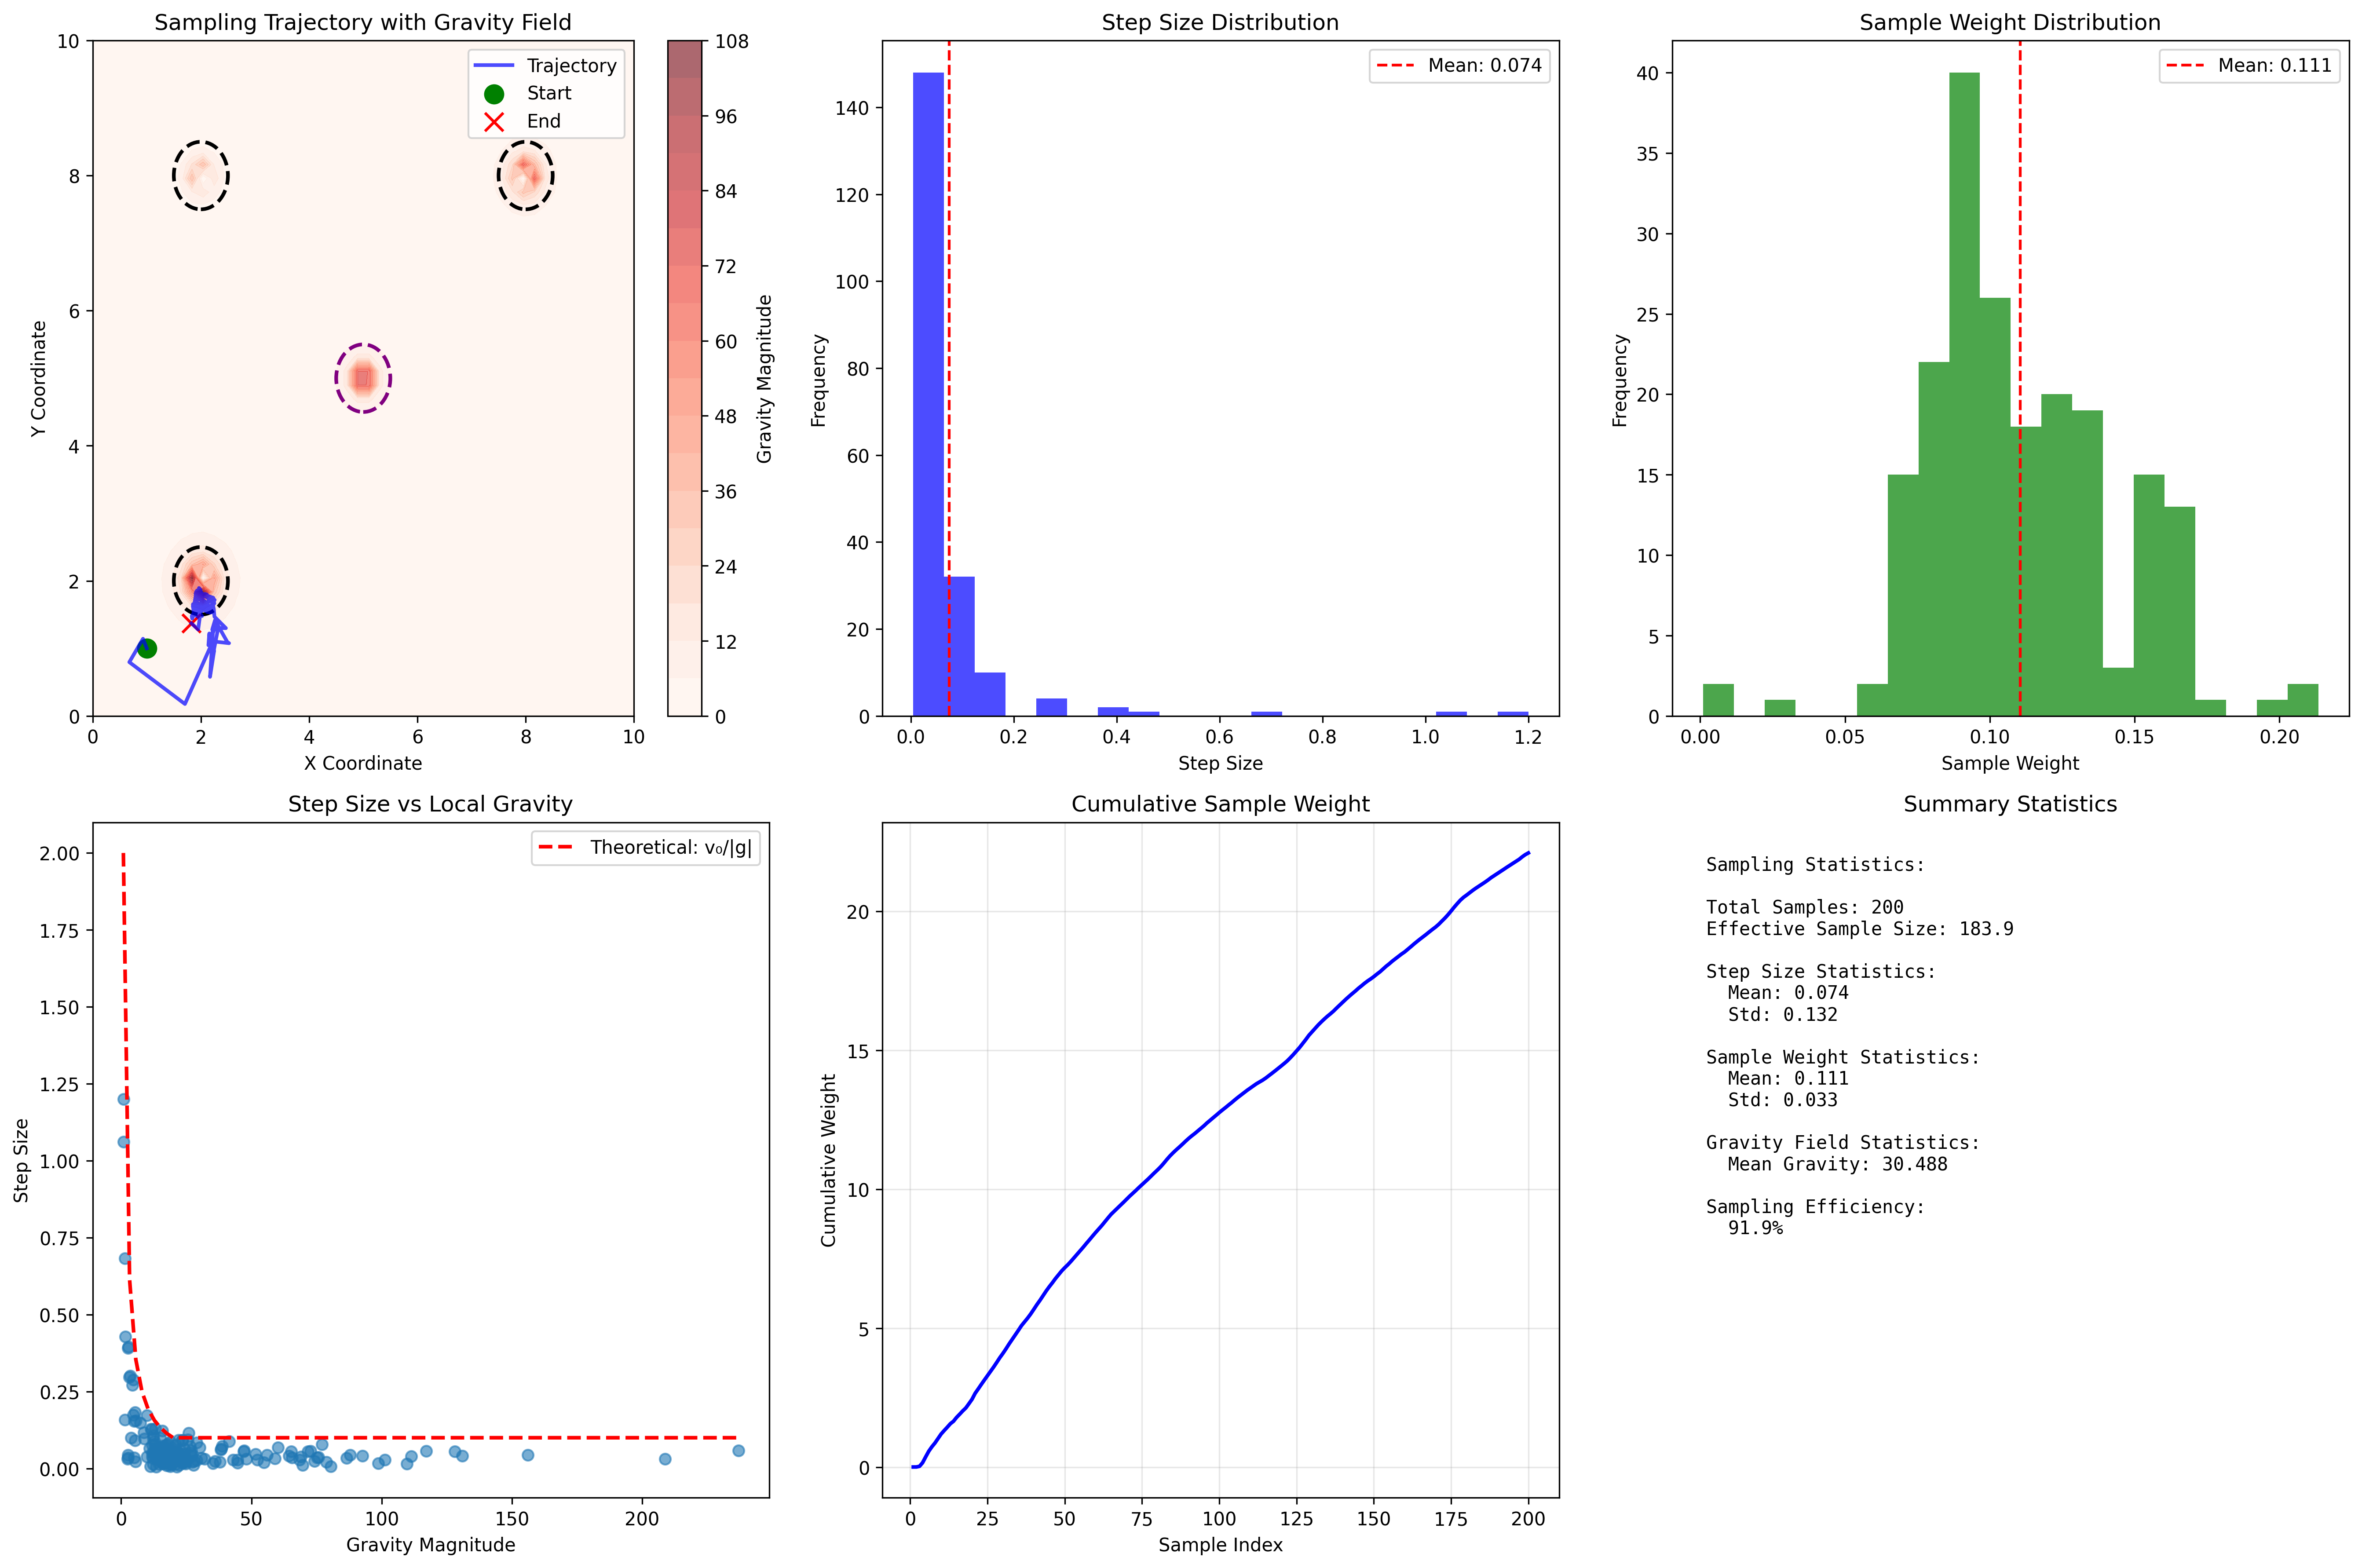
\includegraphics[width=\textwidth]{helicopter/demos/constrained_sampling_demo.png}
\caption{\textbf{Constrained Stochastic Sampling with Semantic Gravity.} Visualization of "pogo stick jump" sampling dynamics in semantic coordinate space. The figure displays: (top left) sampling trajectory overlaid on semantic gravity field contours with attractive (solid circles) and repulsive (dashed circles) gravity zones, (top center) step size distribution showing inverse relationship with local gravity magnitude, (top right) sample weight distribution from fuzzy window aperture functions, (bottom left) step size versus local gravity strength confirming theoretical relationship $\Delta r_{\max} = v_0/\|\mathbf{g}_s\|$, (bottom center) cumulative sample weight evolution indicating sampling efficiency, and (bottom right) summary statistics. The constrained sampling successfully explores high-density semantic regions while respecting local gravity constraints.}
\label{fig:constrained-sampling}
\end{figure}
